\scanpage{21}
\mspage{20}\mspage{10}
\figure{\begin{tikzpicture}\node[draw,ellipse] {$\overline{\underline{\mathrm{VI}}}$};\end{tikzpicture}}
\margin{\uline{Relation avec structure de corps}}
Oublions les structures topologiques, supposons par contre que $R$ ait une \uline{structure de corps}. On supposera alors, \deleted{\unsure{Alrt}} en plus de $(M1)_{\unsure{0}}$ et $(M4)$ (minimum pour construire $\operatorname{Esp}_{\mathcal M_*}$ avec ses $\varprojlim$ finies) l'axiome

\deleted{$(M11)$ \deleted{a) Pour tt} partie modérée $A$ de $R$, l'application $a\mapsto-a$ de $A$ dans $R$ est modérée (i.e. l'ens $\{(a,-a)\in R^2\mid a\in A\}$ est \unsure{modéré|modérée})}

\figure{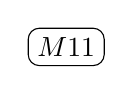
\begin{tikzpicture}\node[draw,rounded corners] {$M11$};\end{tikzpicture}}
a) $0$ et $1$ sont $\in R_0$ i.e. $\{0\},\{1\}\in\mathcal M_1$

b) $\forall A\in\mathcal M_2$, les fonctions
\[
 (x,y)\longmapsto x-y\qquad
 (x,y)\mathrel{\mapstochar\relbar}xy
\]
\deleted{c) $\forall A\subset R^*$, $A\in\mathcal M_1$, $\exists B\in\mathcal M_1$ tel que $A^{-1}\subset B$}
\margin{\deleted{(\unsure{car|OPS} OPS $B=A^{-1}$\,!)}}
sur $A$ sont modérées, \deleted{\unsure{car}} i.e. les deux parties de $R^3$
\[
 \{(x,y,x-y)\mid(x,y)\in A\},\qquad\text{et }\{(a,y,xy)\mid(x,y)\in A\}
\]
sont modérées.

c) $\forall A\subset R^*$, $A\in\mathcal M_1$, $\exists B\in\mathcal M_1$ avec $A^{-1}$ \deleted{modérée}\inserted{$\subset B$} (OPS $B=A^{-1}$\,!).

\deleted{Cet axiome} \deleted{\unsure{les parties a) b)}} \inserted{les parties a) b)} \unsure{équivalent|équivaut} à la validité de la

\margin{\uline{NB} Si $R\in\mathcal M_1$, il suffit de prendre $(M11)$ pour $A=R^2$}

\uline{Proposition} Pour un espace modéré $X$, les fonctions modérées $X\mathbin{-}R$ \deleted{\unsure{et|est} = une sous $R_0$} forment un \uline{sous-anneau} de l'anneau des fonctions scalaires sur $X$. En particulier, $R_0$ est un sous-anneau de $R$, et les anneaux
\margin{de fonctions mod. sont des $R_0$-algèbres}
